% Digital Logic Report Template
% Created: 2020-01-10, John Miller

%==========================================================
%=========== Document Setup  ==============================

% Formatting defined by class file
\documentclass[11pt]{article}

% ---- Document formatting ----
\usepackage[margin=1in]{geometry}	% Narrower margins
\usepackage{booktabs}				% Nice formatting of tables
\usepackage{graphicx}				% Ability to include graphics

%\setlength\parindent{0pt}	% Do not indent first line of paragraphs 
\usepackage[parfill]{parskip}		% Line space b/w paragraphs
%	parfill option prevents last line of pgrph from being fully justified

% Parskip package adds too much space around titles, fix with this
\RequirePackage{titlesec}
\titlespacing\section{0pt}{8pt plus 4pt minus 2pt}{3pt plus 2pt minus 2pt}
\titlespacing\subsection{0pt}{4pt plus 4pt minus 2pt}{-2pt plus 2pt minus 2pt}
\titlespacing\subsubsection{0pt}{2pt plus 4pt minus 2pt}{-6pt plus 2pt minus 2pt}

% ---- Hyperlinks ----
\usepackage[colorlinks=true,urlcolor=blue]{hyperref}	% For URL's. Automatically links internal references.

% ---- Code listings ----
\usepackage{listings} 					% Nice code layout and inclusion
\usepackage[usenames,dvipsnames]{xcolor}	% Colors (needs to be defined before using colors)

% Define custom colors for listings
\definecolor{listinggray}{gray}{0.98}		% Listings background color
\definecolor{rulegray}{gray}{0.7}			% Listings rule/frame color

% Style for Verilog
\lstdefinestyle{Verilog}{
	language=Verilog,					% Verilog
	backgroundcolor=\color{listinggray},	% light gray background
	rulecolor=\color{blue}, 			% blue frame lines
	frame=tb,							% lines above & below
	linewidth=\columnwidth, 			% set line width
	basicstyle=\small\ttfamily,	% basic font style that is used for the code	
	breaklines=true, 					% allow breaking across columns/pages
	tabsize=3,							% set tab size
	commentstyle=\color{gray},	% comments in italic 
	stringstyle=\upshape,				% strings are printed in normal font
	showspaces=false,					% don't underscore spaces
}

% How to use: \Verilog[listing_options]{file}
\newcommand{\Verilog}[2][]{%
	\lstinputlisting[style=Verilog,#1]{#2}
}




%======================================================
%=========== Body  ====================================
\begin{document}

\title{ELC 2137 Lab 3: Adders}
\author{Victoria Covey}

\maketitle


\section*{Summary}

In this lab we experimented with carries and sums that are produced in binary adders. We created 3 circuits, all of which came together to make our final 2-bit adder. To prove the circuits and binary calculations the circuit was making were true, the class made sperate schematics, wiring diagrams, and truth tables. After this lab, I felt more confident in my ability to read and write a circuit schematic, as well as how to use transistors to make calculations of And and XOR gates.

\section*{Q\&A}
\begin{enumerate}
	\item Which gates could we use for combining the carry bits?
	
	We could use AND and XOR gates as we had seen in class.
	
	\item Which of the above should we use and why?
	
	We would want to use the AND gates. The AND gates can be negated in a way that mimics the use of XOR without adding another transistor chip.

\end{enumerate}

\section*{Results}
\begin{center}

	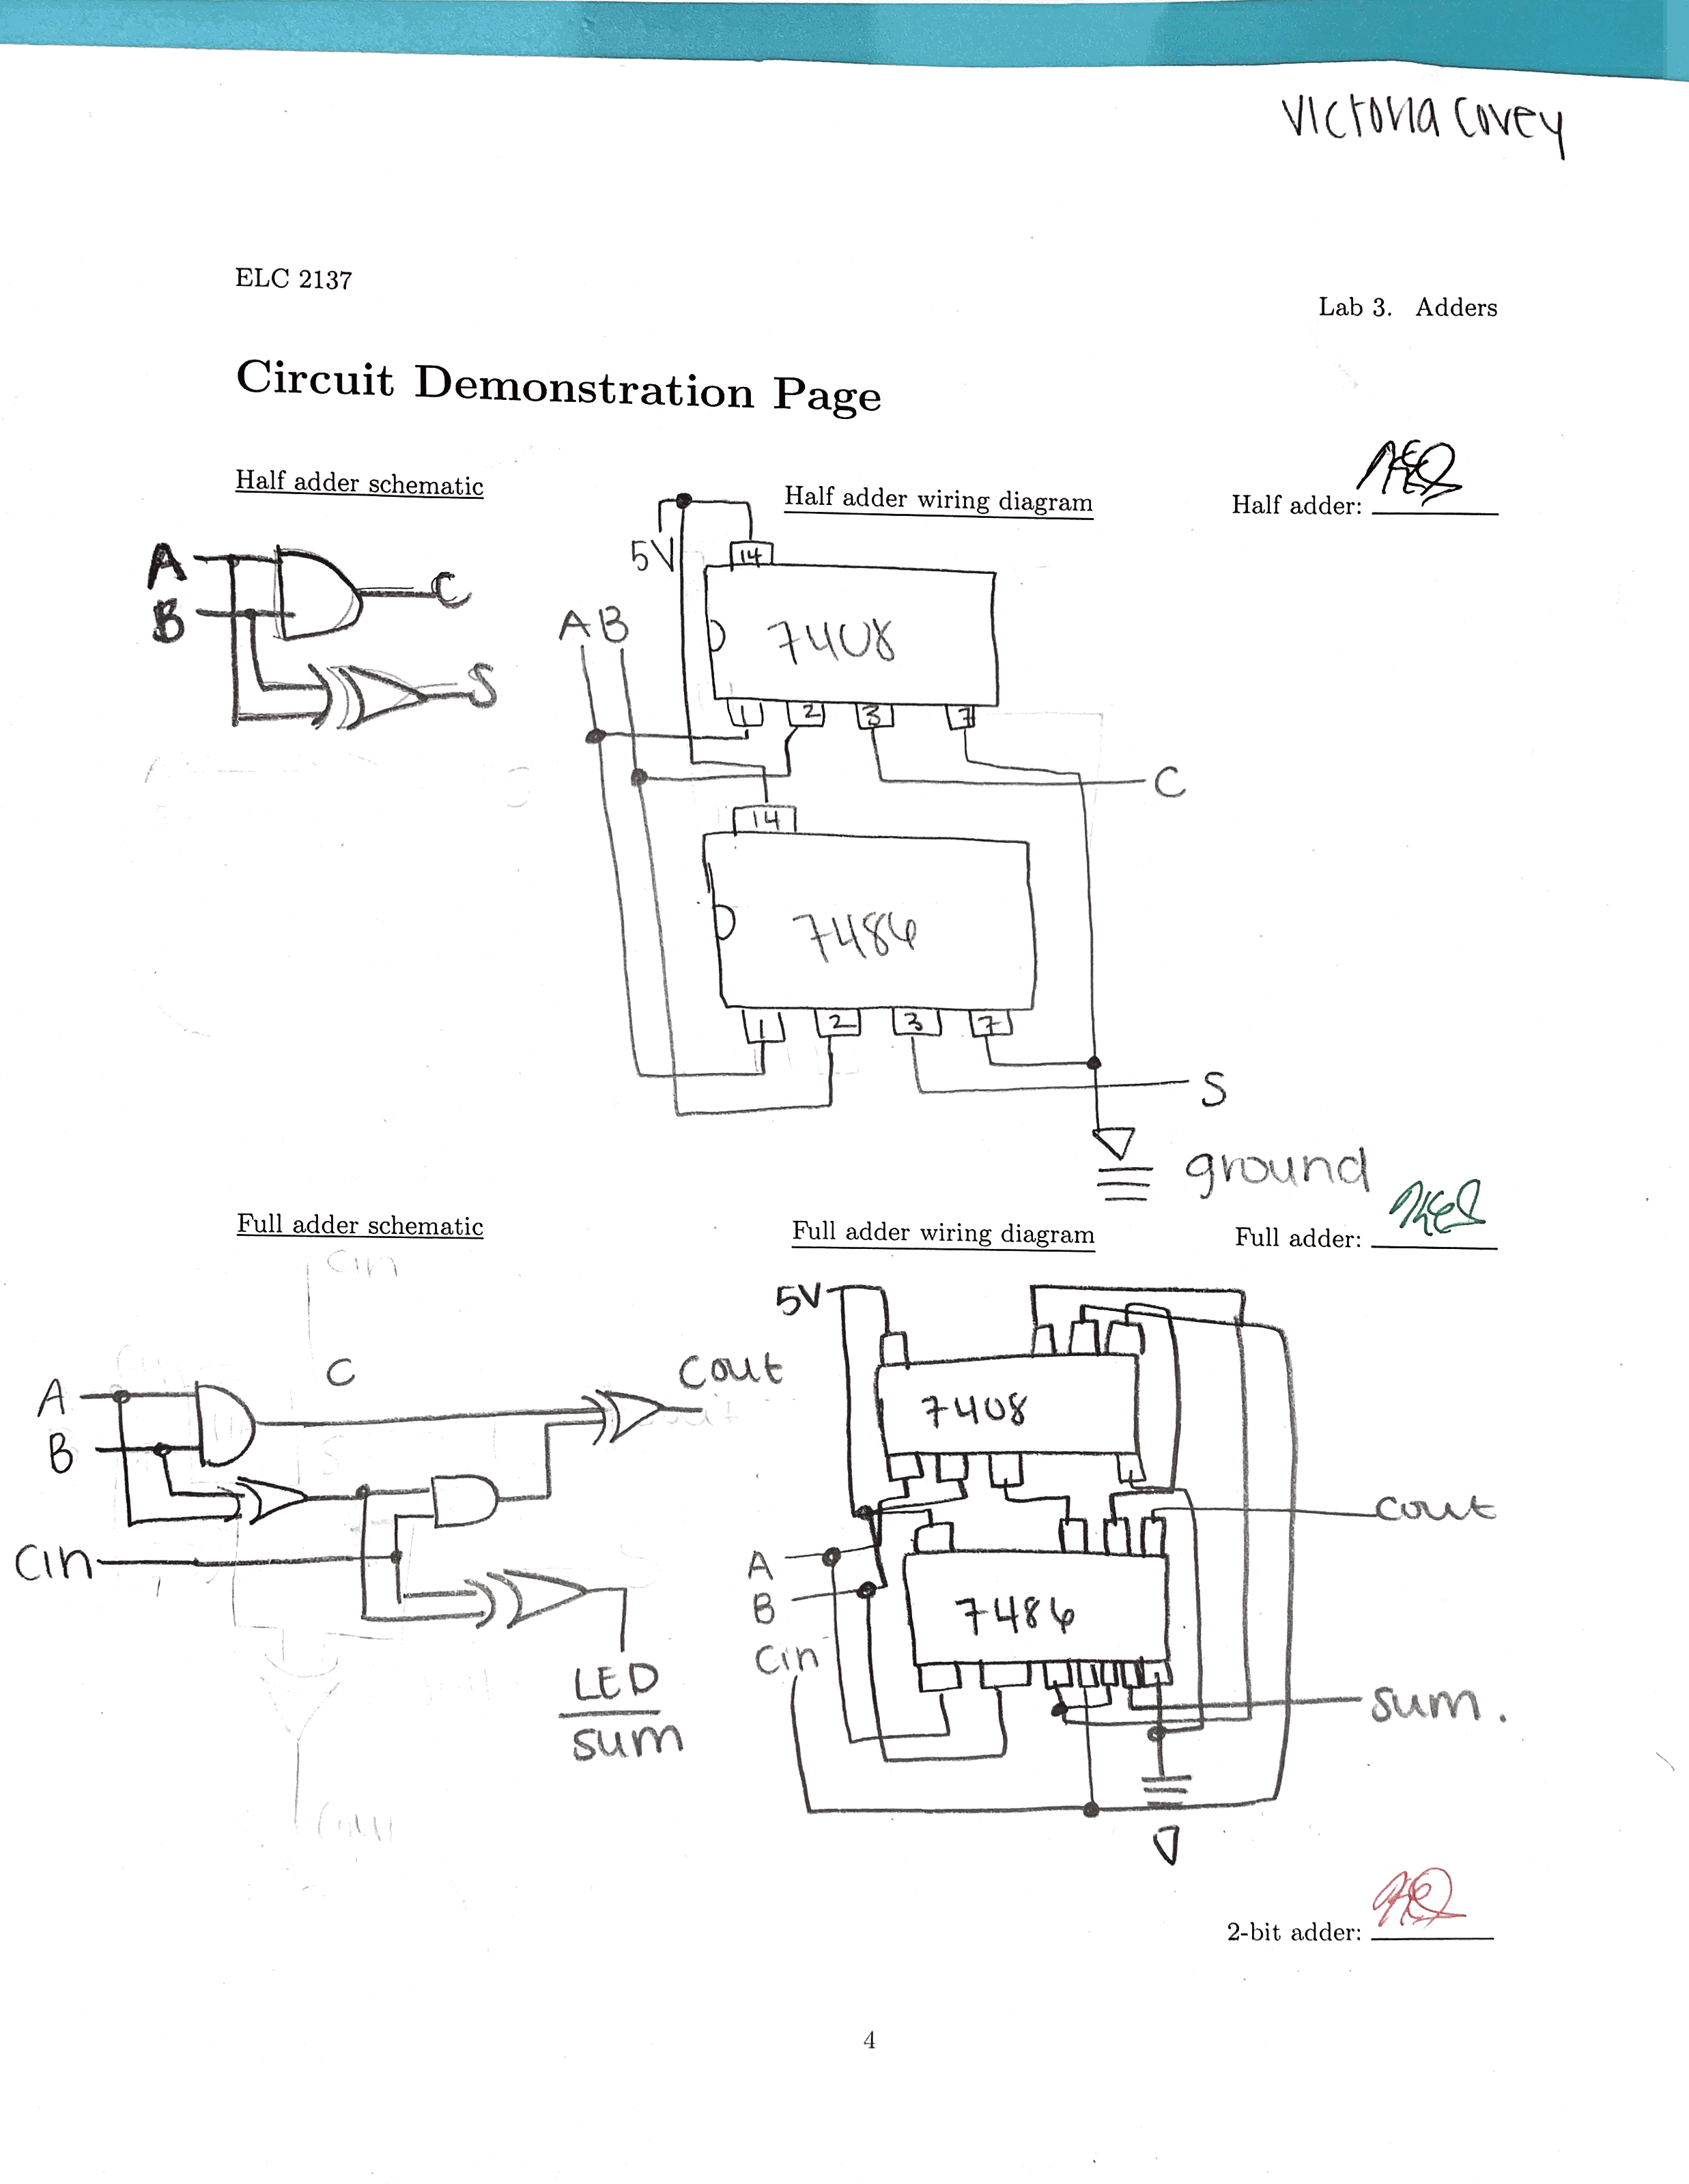
\includegraphics[width=0.8\textwidth,trim=0cm 6cm 0.6cm 4cm,clip]{Circuit_Demonstration}

\caption{fig: Signed Off Circuit Demonstration Page}

	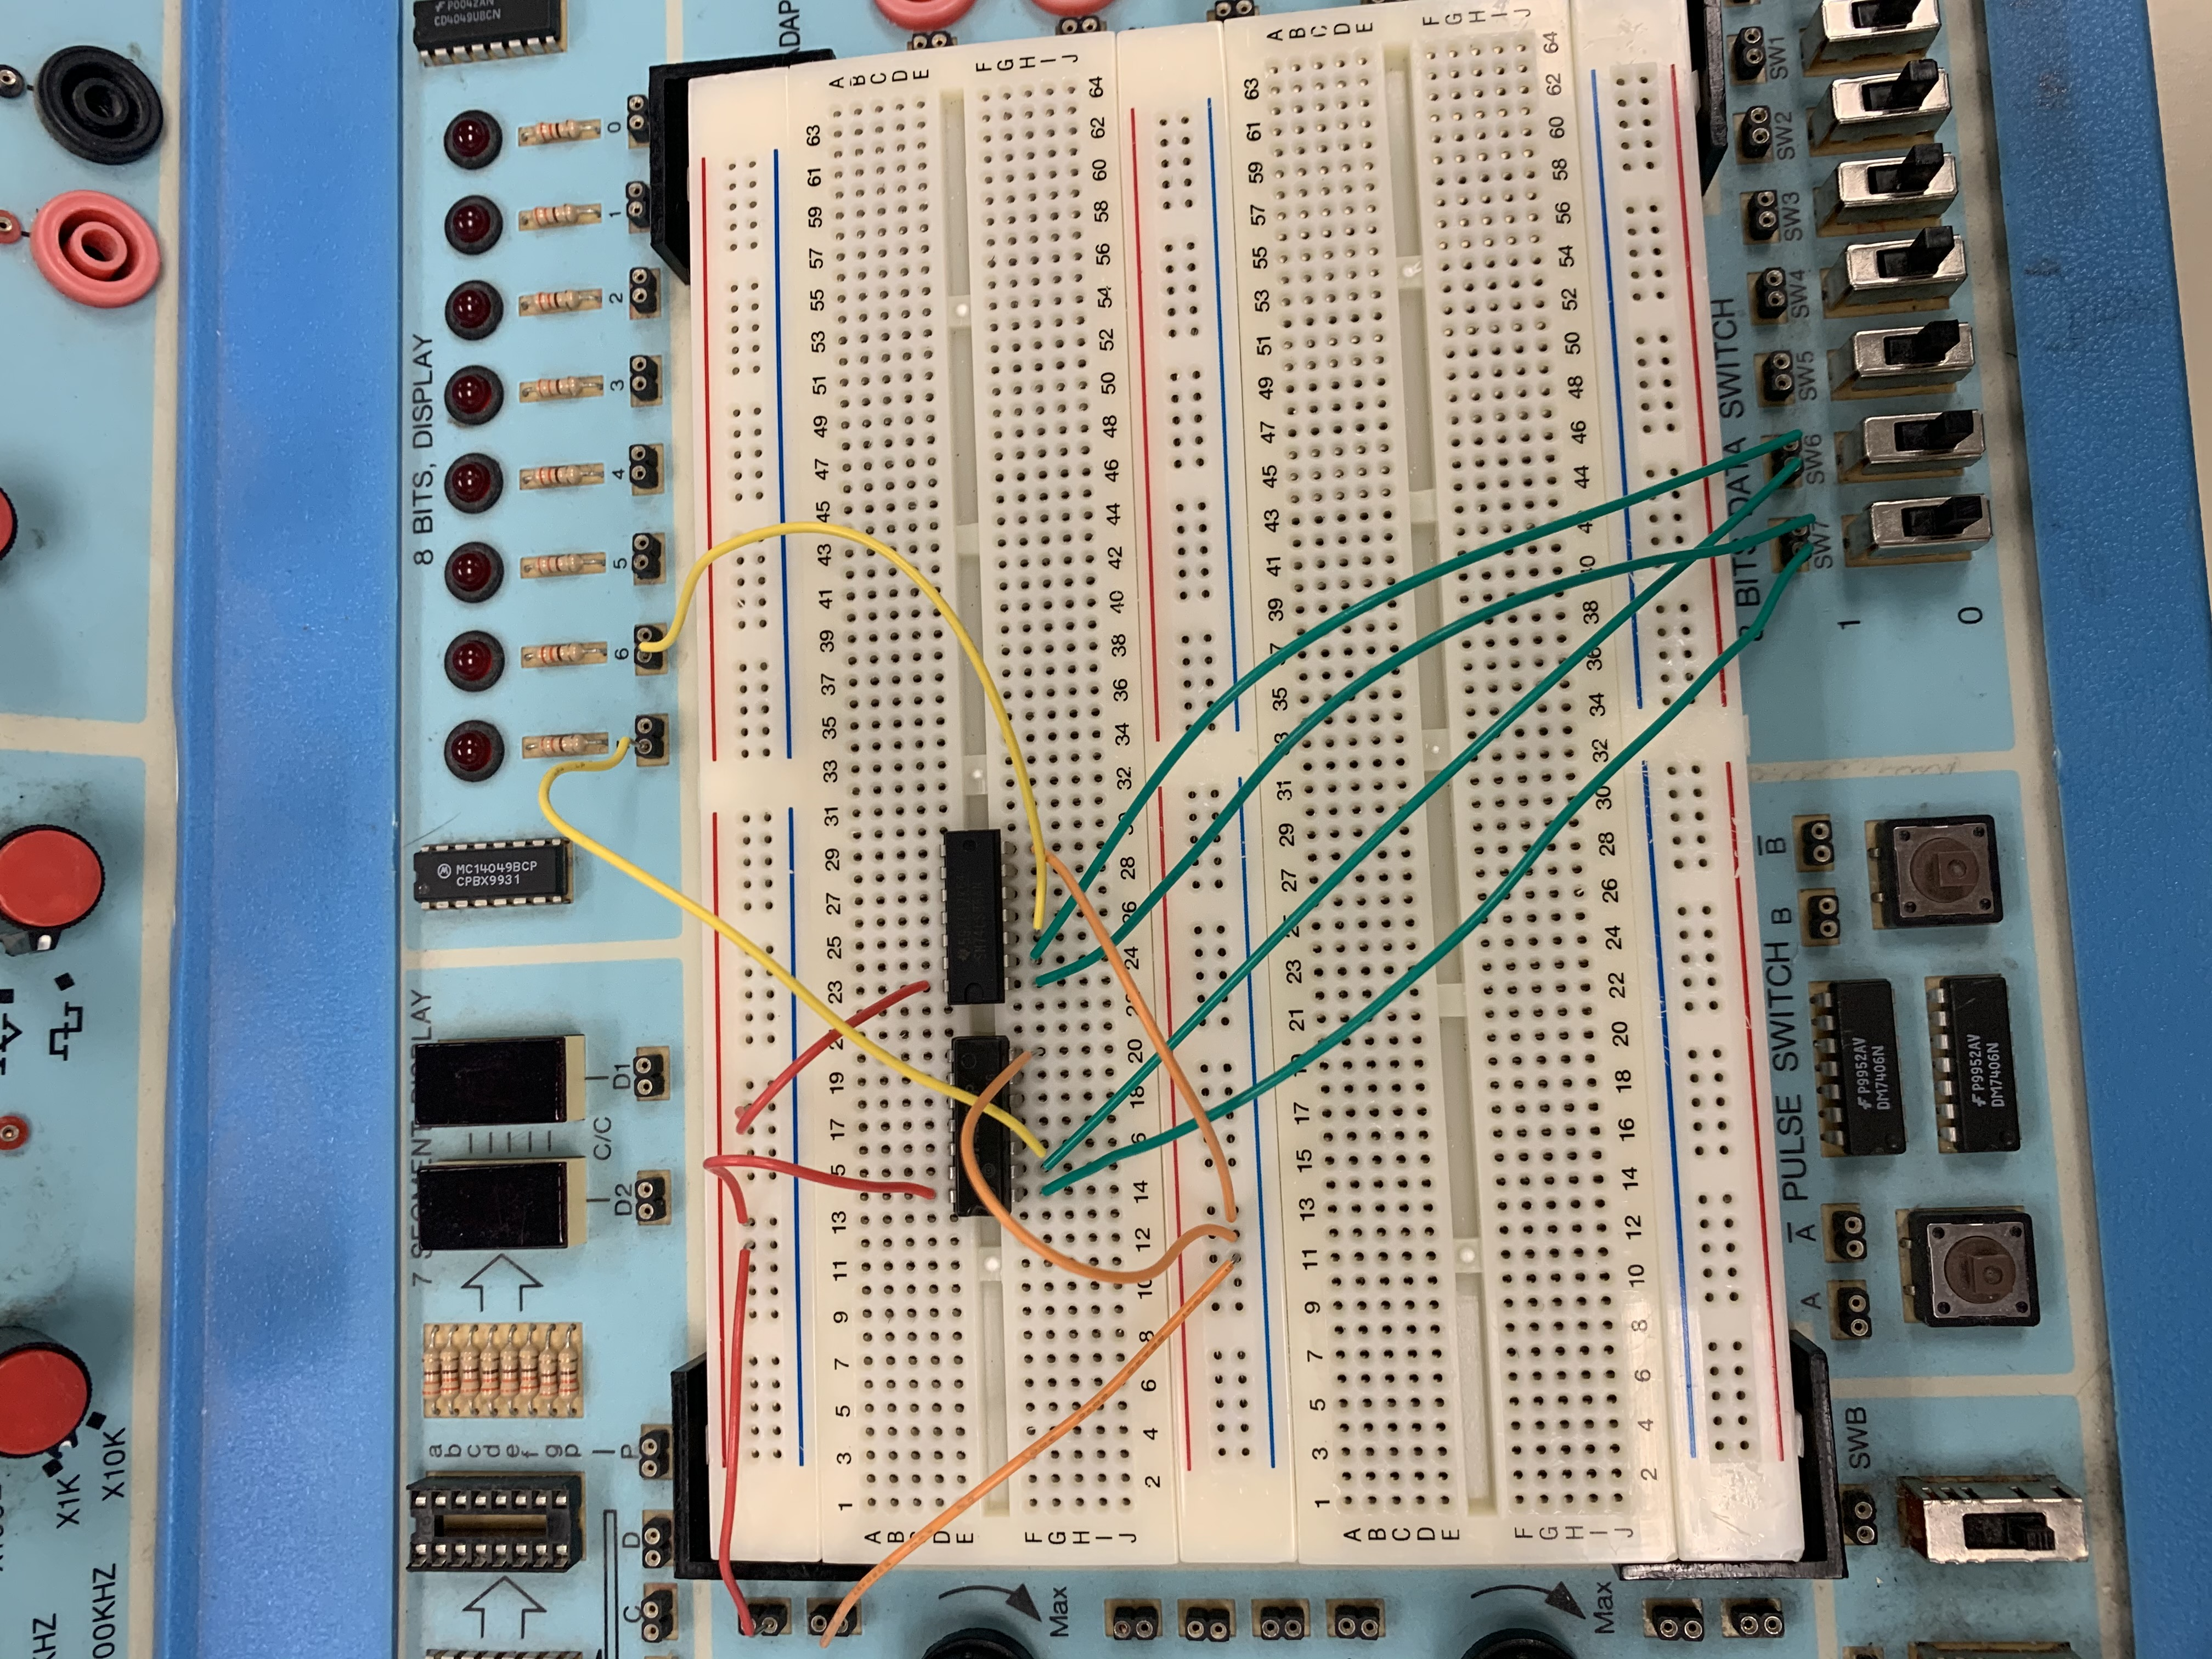
\includegraphics[width=0.8\textwidth,trim=0cm 0cm 0.6cm 0cm,clip]{HA}
	
\caption{fig: Half Adder Circuit}
	
	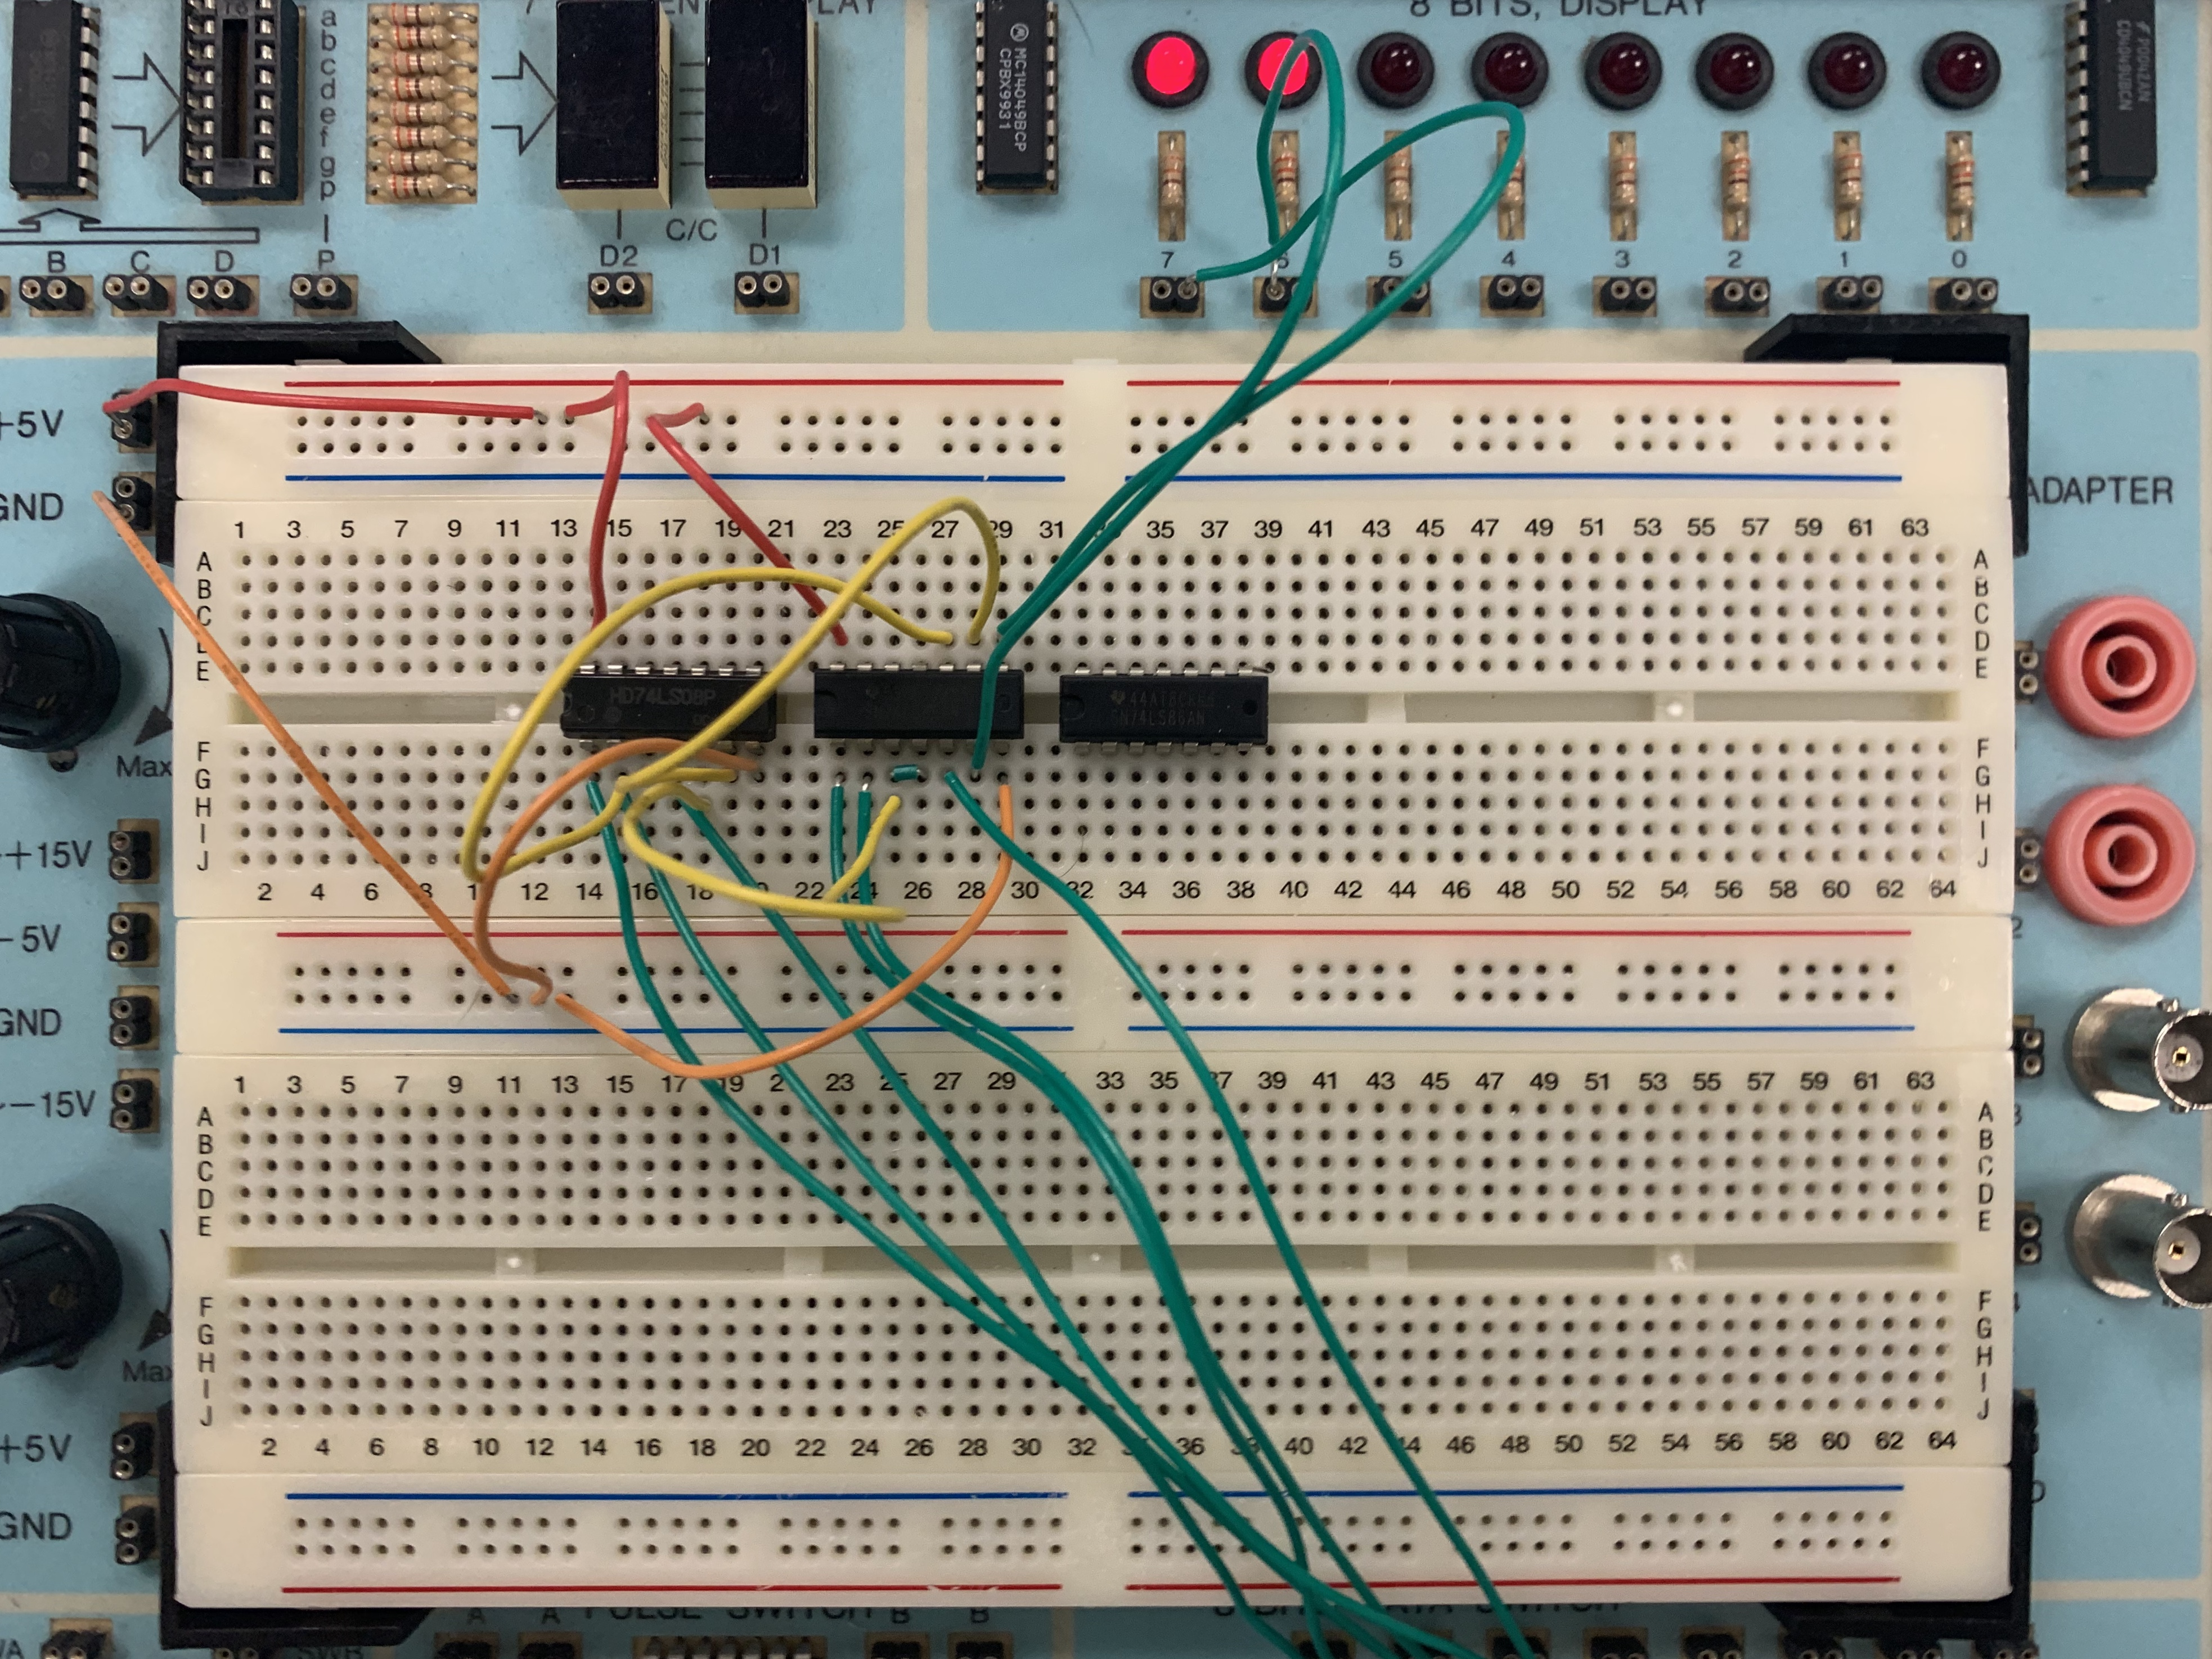
\includegraphics[width=0.8\textwidth,trim=0cm 0cm 0.6cm 0cm,clip]{FA}
	
\caption{fig: Full Adder Circuit}

	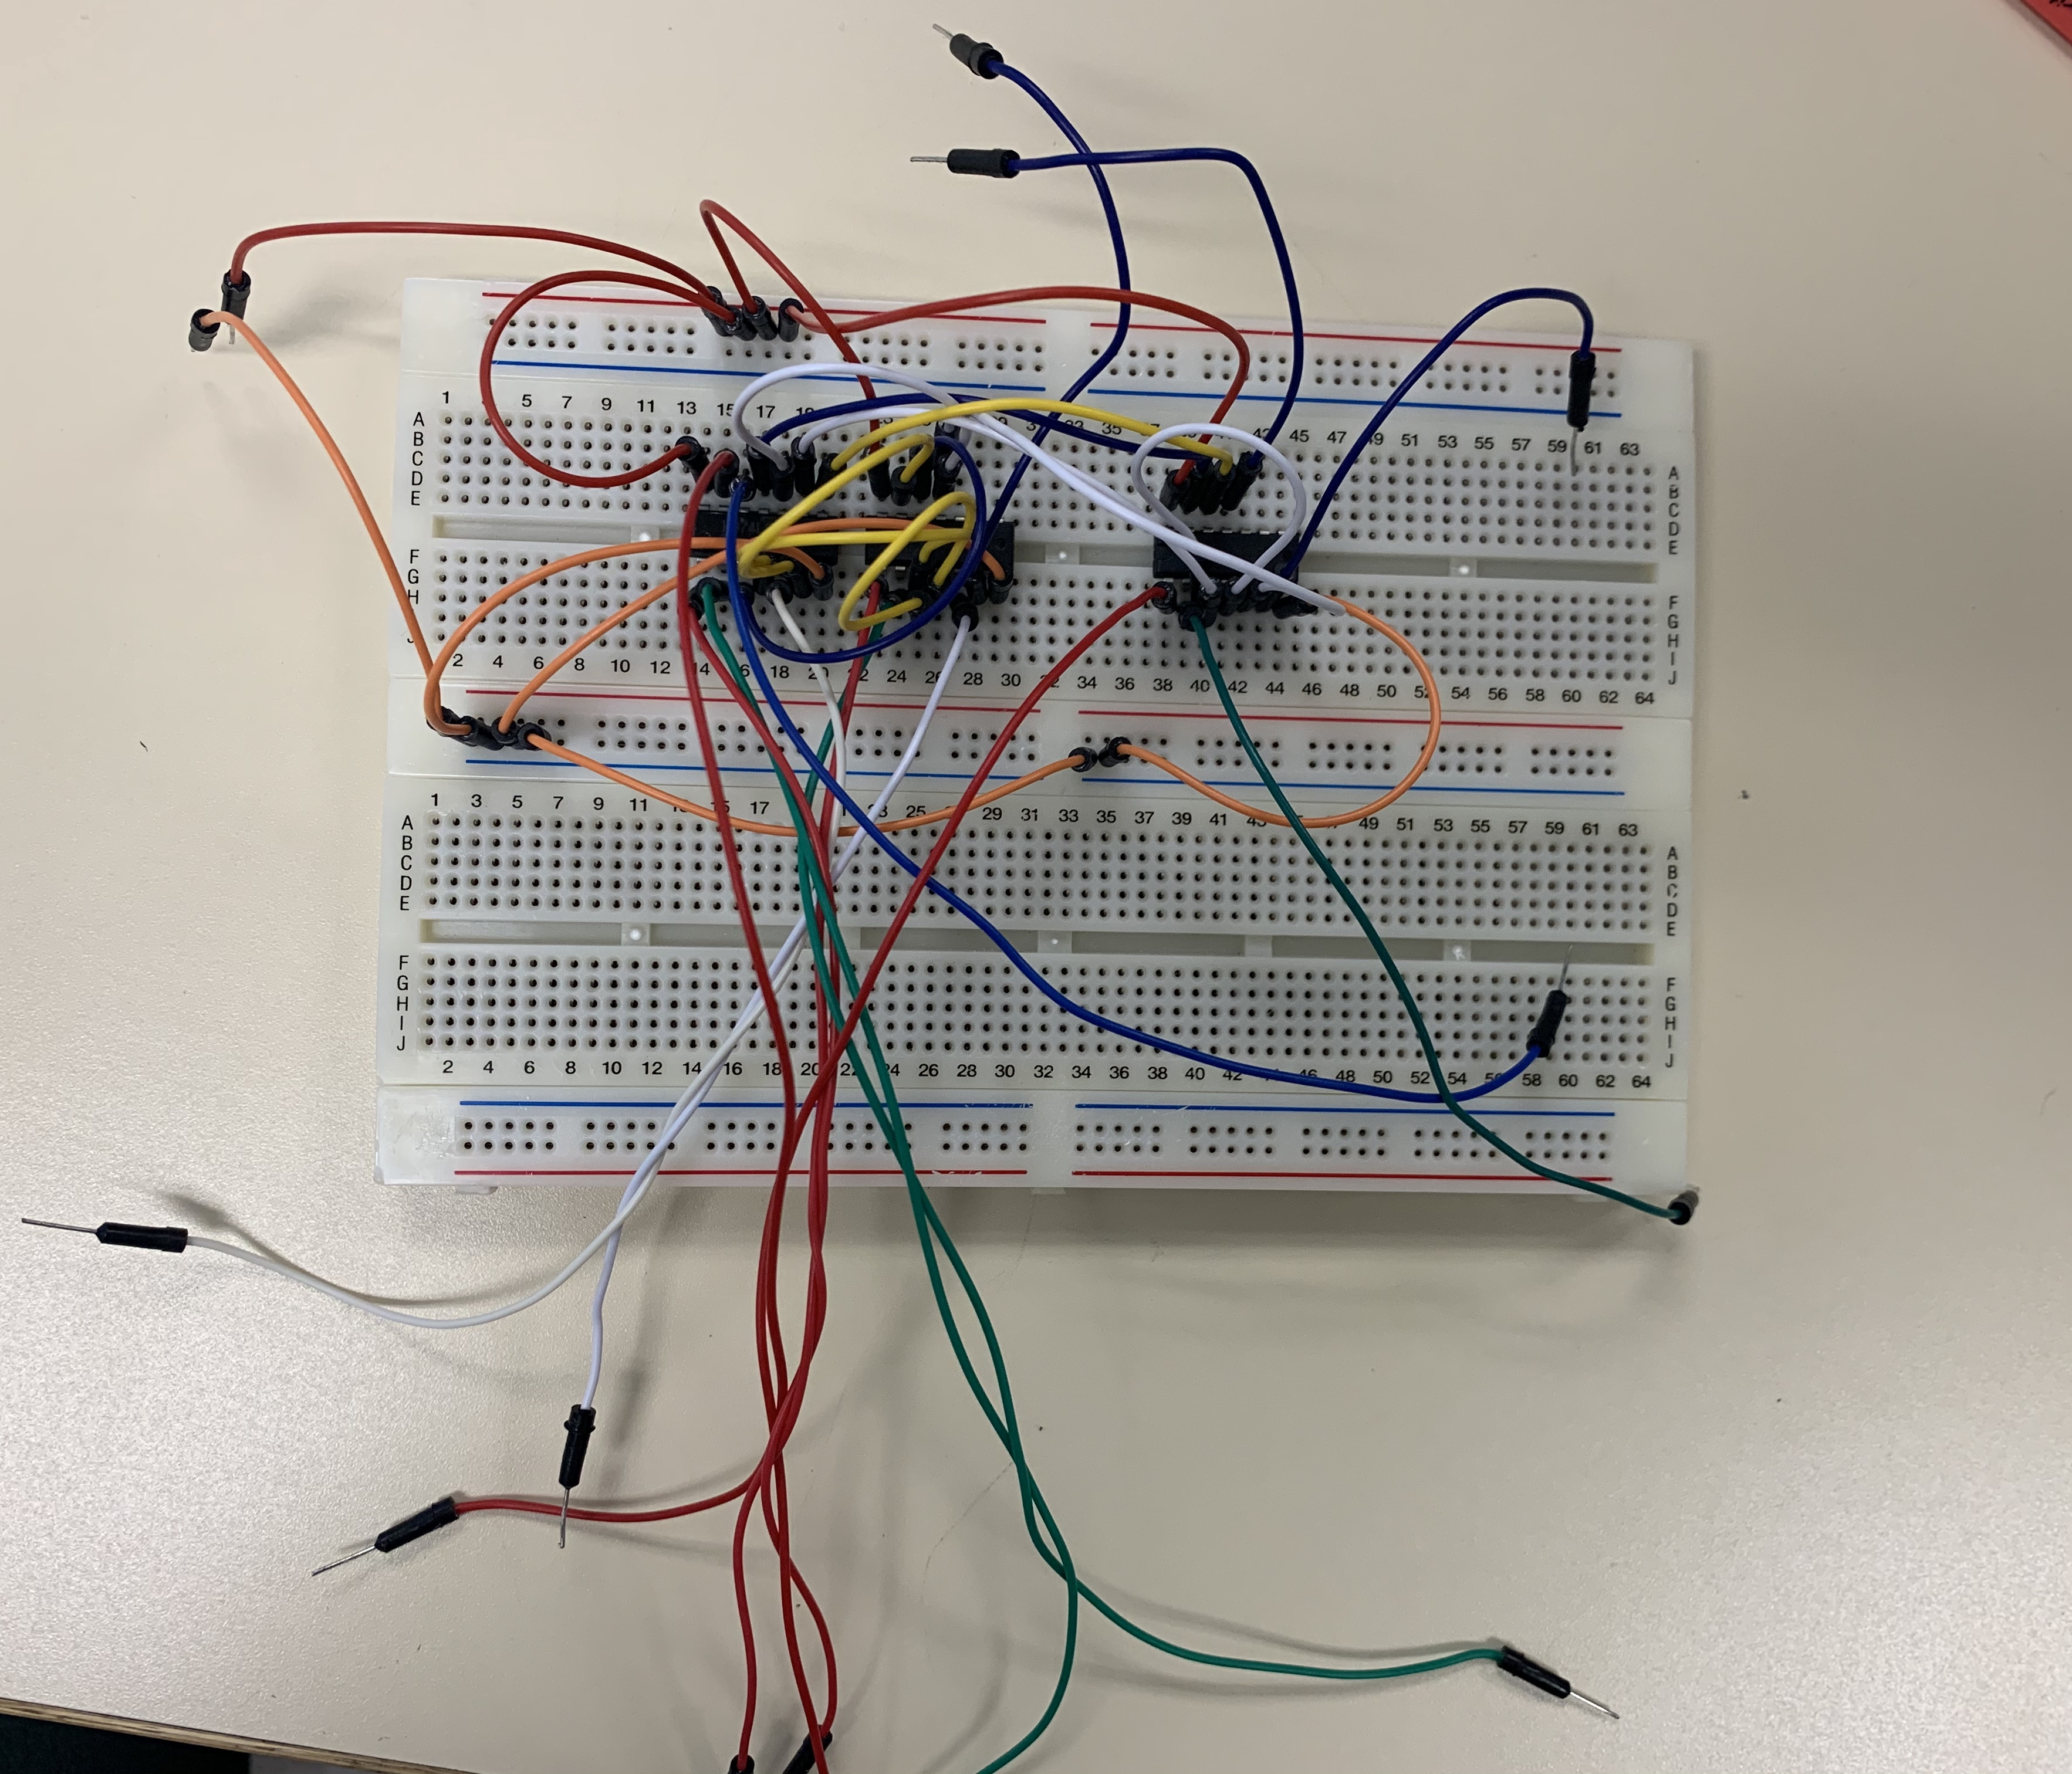
\includegraphics[width=0.8\textwidth,trim=0cm 0cm 0.6cm 0cm,clip]{2BA}
	
\caption{fig: 2 Bit Adder Circuit}
	
	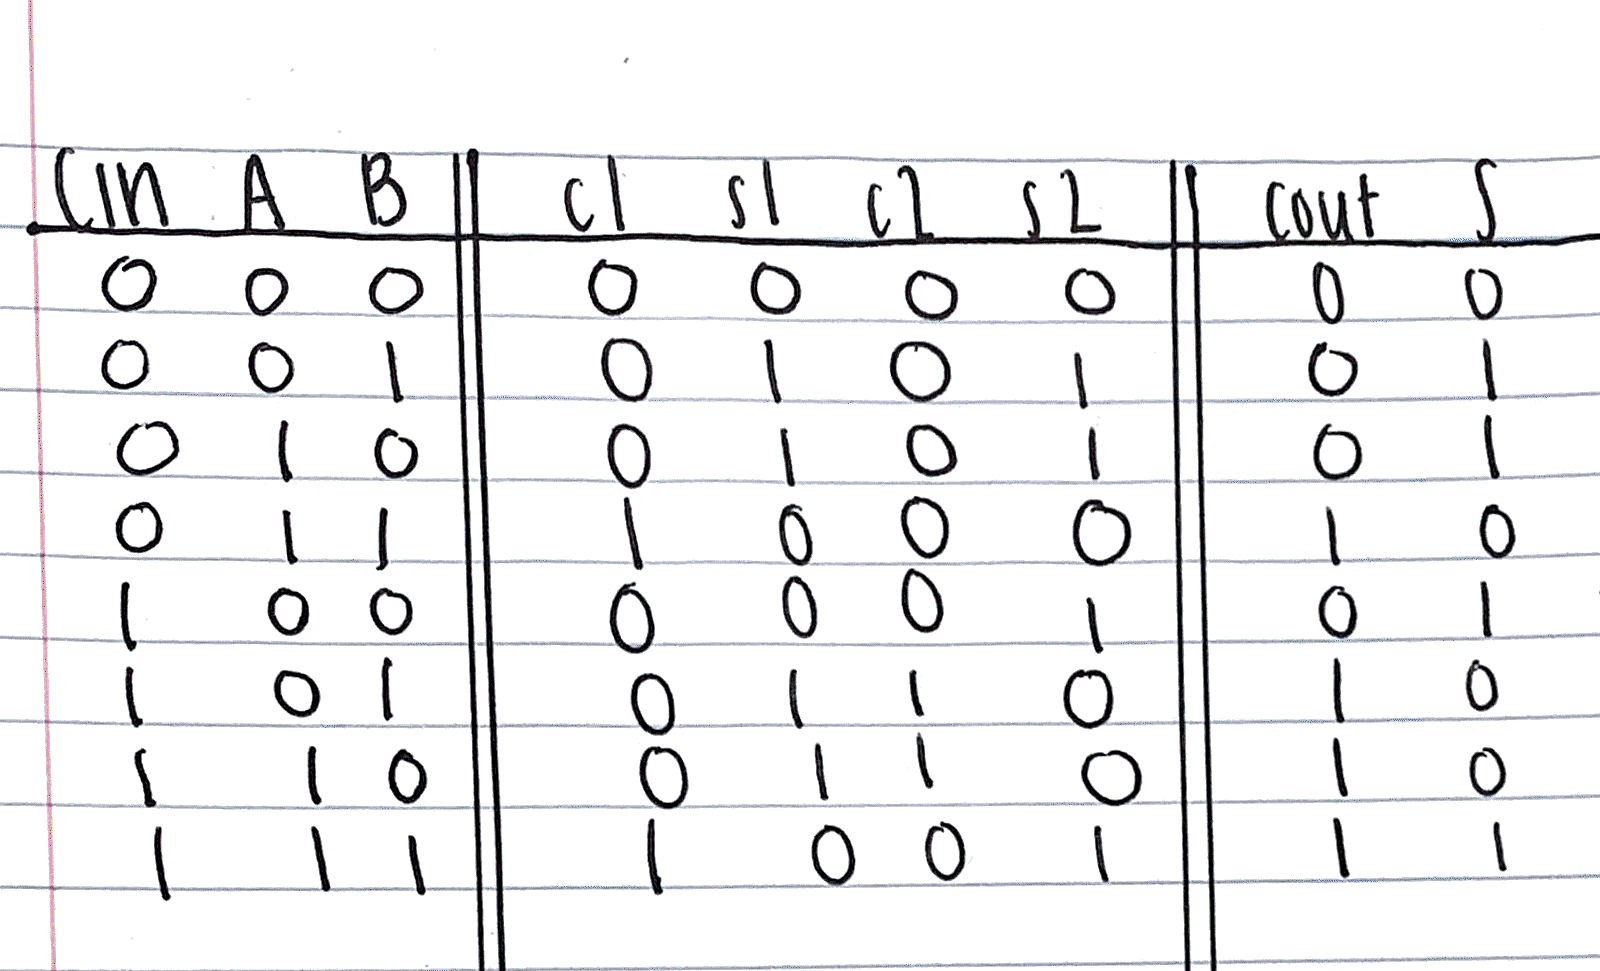
\includegraphics[width=0.8\textwidth,trim=0cm 0cm 0.6cm 0cm,clip]{HATruth}
	
\caption{fig: Full Adder Truth Table Showing Half Adders}
	
\end{center}
\end{document}
